\documentclass[a4paper,12pt]{article}
\usepackage{HomeWorkTemplate}
\usepackage{circuitikz}
\usepackage[shortlabels]{enumitem}
\usepackage{float}
\usepackage{hyperref}
\usepackage{tikz}
\usepackage{amsmath}
\usepackage{amssymb}
\usepackage{tcolorbox}
\usepackage{xepersian}
\settextfont{XB Niloofar}
\usetikzlibrary{arrows,automata}
\usetikzlibrary{circuits.logic.US}
\usepackage{changepage}
\newcounter{problemcounter}
\newcounter{subproblemcounter}
\setcounter{problemcounter}{1}
\setcounter{subproblemcounter}{1}
\newcommand{\problem}[1]
{
	\subsection*{
		پرسش
		\arabic{problemcounter} 
		\stepcounter{problemcounter}
		\setcounter{subproblemcounter}{1}
		#1
	}
}
\newcommand{\subproblem}{
	\textbf{\harfi{subproblemcounter})}\stepcounter{subproblemcounter}
}


\begin{document}
\handout
{آز طراحی سیستم‌های دیجیتال}
{دکتر سیاوش بیات سرمدی}
{نیم‌سال اول 1400\lr{-}1401}
{اطلاعیه}
{ \newline حسین آقایی \newline پرهام چاوشیان}
{\newline 98105619 \newline 98100118 }
 {گزارش آزمایش پنجم}
{خانم زینب رشیدی}
تنها یک ماژول داریم که همان ماژول انکوباتور است. 3 استیت برای روشن یا خاموش بودن کولر و هیتر تعریف کرده‌ایم. 4 استیت نیز برای تعداد دور فن تعریف کرده‌ایم. در صورت آمدن سیگنال ریست به استیت اول می‌رویم. در هر مرحله باتوجه به استیت فعلی و دمای ورودی، استیت بعدی را تعیین می‌کنیم(هم برای کولر و هیتر و هم برای فن). در نهایت باتوجه به استیتی که در آن هستیم، خروجی روشن یا خاموش بودن کولر و همچنین دور فن را تعیین می‌کنیم.\\
نتایج شبیه‌سازی نیز در ادامه آمده است، دقت کنید که خروجی تنها در پالس ساعتی که خروجی $done$ برابر 1 شده است، معتبر است. (در صورت نیاز تصاویر به طور جداگانه نیز پیوست شده اند):
\begin{figure}[H]
 \centering
  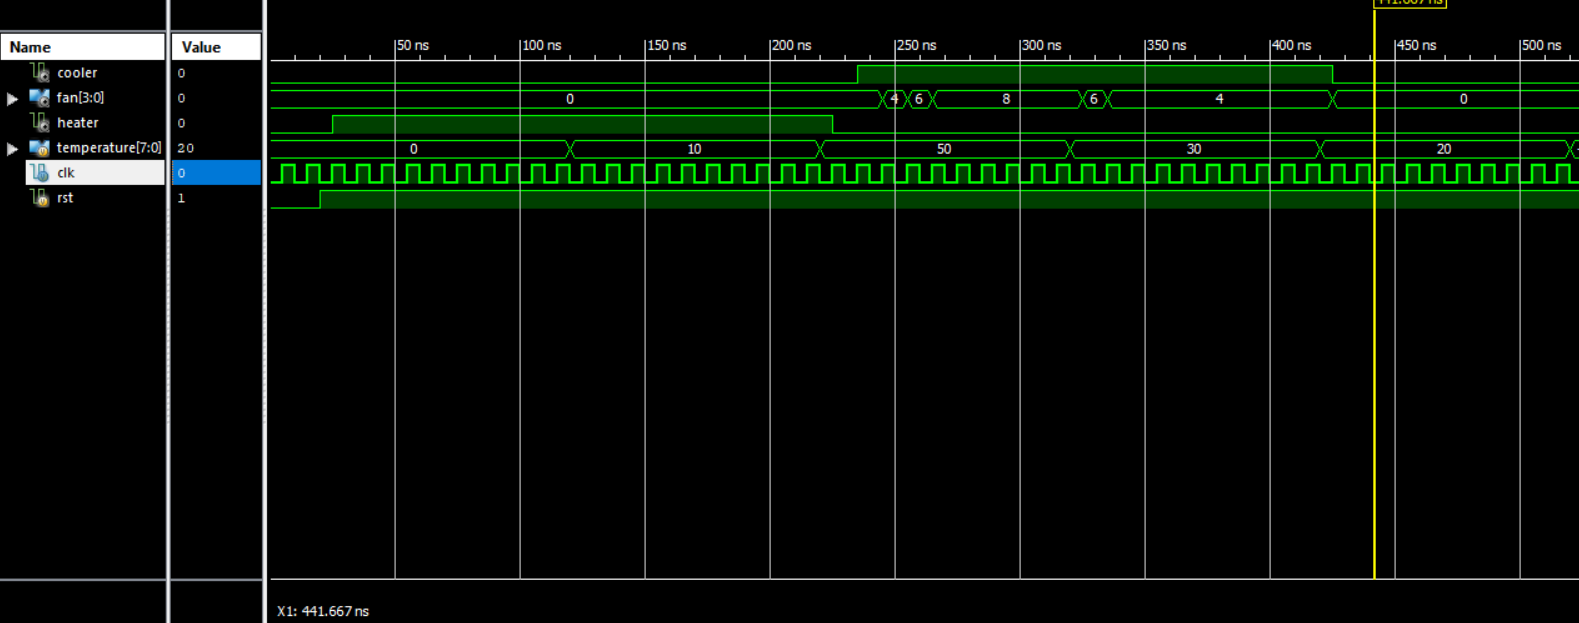
\includegraphics[width=0.8\linewidth]{s1}
\end{figure}
\begin{figure}[H]
 \centering
  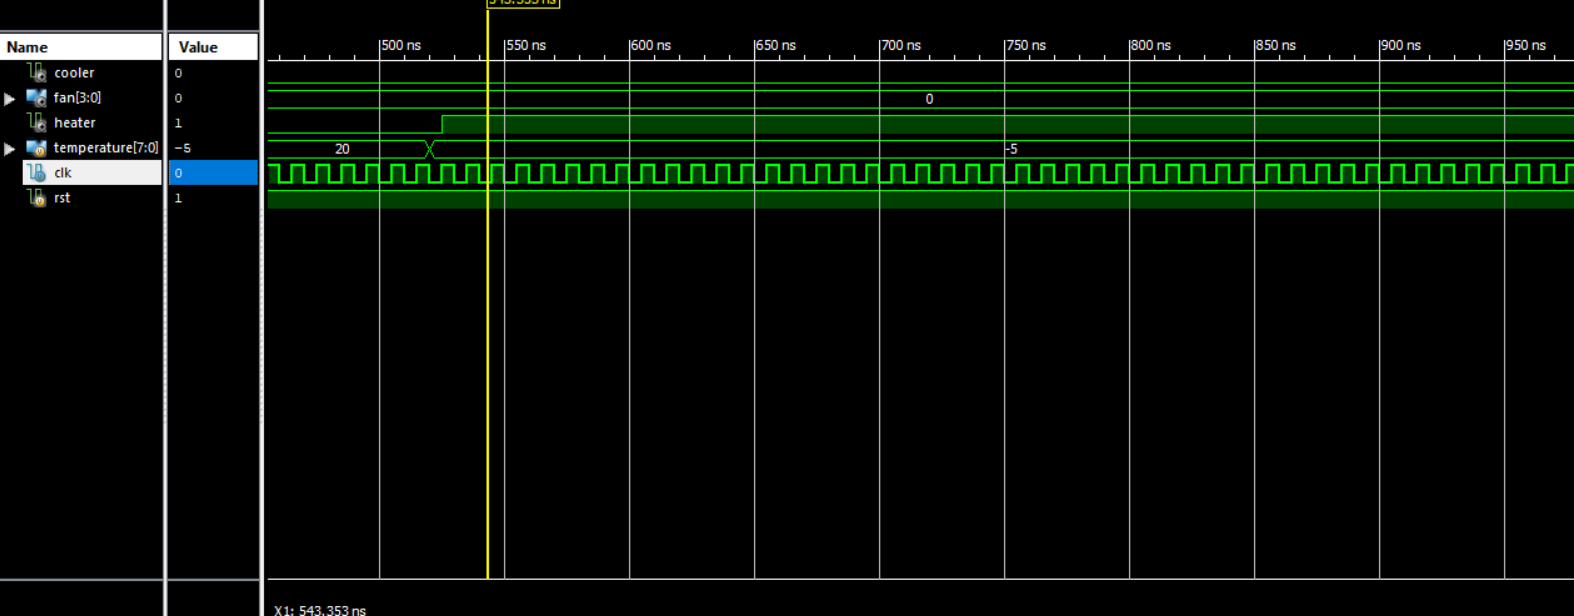
\includegraphics[width=0.8\linewidth]{s2}
\end{figure}
\end{document}
